\documentclass[border=2pt]{standalone}
\usepackage[dvipsnames,svgnames,x11names]{xcolor}
\usepackage{tikz}
\usetikzlibrary{arrows.meta,shapes.geometric}
\begin{document}
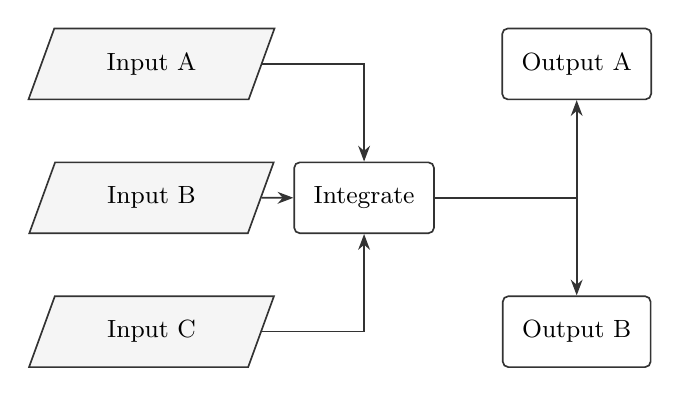
\begin{tikzpicture}[font=\small,>=Stealth,x=27mm,y=17mm]
\node[trapezium,trapezium left angle=70,trapezium right angle=110,fill=black!4,draw=black!80,text=black,line width=0.6pt,minimum height=9mm,inner xsep=7pt,inner ysep=4.5pt,align=center] (in-a) at (0,0) {Input A};
\node[trapezium,trapezium left angle=70,trapezium right angle=110,fill=black!4,draw=black!80,text=black,line width=0.6pt,minimum height=9mm,inner xsep=7pt,inner ysep=4.5pt,align=center] (in-b) at (0,-1) {Input B};
\node[trapezium,trapezium left angle=70,trapezium right angle=110,fill=black!4,draw=black!80,text=black,line width=0.6pt,minimum height=9mm,inner xsep=7pt,inner ysep=4.5pt,align=center] (in-c) at (0,-2) {Input C};
\node[rectangle,rounded corners=2pt,fill=white,draw=black!80,text=black,line width=0.6pt,minimum height=9mm,inner xsep=7pt,inner ysep=4.5pt,align=center] (merge) at (1,-1) {Integrate};
\node[rectangle,rounded corners=2pt,fill=white,draw=black!80,text=black,line width=0.6pt,minimum height=9mm,inner xsep=7pt,inner ysep=4.5pt,align=center] (out-a) at (2,0) {Output A};
\node[rectangle,rounded corners=2pt,fill=white,draw=black!80,text=black,line width=0.6pt,minimum height=9mm,inner xsep=7pt,inner ysep=4.5pt,align=center] (out-b) at (2,-2) {Output B};
\draw[->,draw=black!80,line width=0.6pt] (in-a) -| (merge);
\draw[->,draw=black!80,line width=0.6pt] (in-b) -- (merge);
\draw[->,draw=black!80,line width=0.6pt] (in-c) -| (merge);
\draw[->,draw=black!80,line width=0.6pt] (merge) -| (out-a);
\draw[->,draw=black!80,line width=0.6pt] (merge) -| (out-b);
\end{tikzpicture}
\end{document}
